\subsection{Ondas estacionárias de som em um gás nobre
desconhecido}

Nesse experimento, nós utilizaremos o mesmo aparato dos experimentos anteriores (Tubo de Kundt), para medirmos a velocidade do som, agora, em um gás desconhecido. Tendo a velocidade do som nesse meio, podemos estimar qual é o gás ali presente.\\

Usaremos uma frequência de excitação fixa – da ordem de 2 kHz – e vamos variando o comprimento \textbf{L} da coluna do gás desconhecido, de modo a obter o primeiro harmônico.\\

Dessa forma, obteremos uma relação entre a velocidade do som no gás desconhecido \textbf{v}, a frequência do primeiro harmônico \textbf{$f_1$} e o comprimento da coluna de gás \textbf{L}:

\[v = 2\cdot L\cdot f_1\]

Com base no vídeo, podemos encontrar o comprimento da coluna de gás em que se forma o primeiro harmônico, e sabemos que é 23cm ou 0,23m.

\[L = 0,230 \pm 0,001 m\]

Utilizando a fórmula destacada acima, vamos encontrar a velocidade:

\[ v = 2\cdot L \cdot f_1   =   2\cdot(0,230)\cdot 2\cdot 10^3\]

\[v = 920 m/s\]

Calcularemos, também, sua incerteza:

\[\delta _v = 2 \cdot \delta _L \cdot f1   =   2\cdot(0,001)\cdot2\cdot10^3\]
\[\delta _v = 4 m/s\]
Desse modo, nossa velocidade pode ser expressa como:
\[v = 920 \pm 4 m/s\]

Desse modo, procuramos em literaturas as velocidades do som em diferentes gases, para encontrarmos qual seria o gás desconhecido do experimento. Nos baseamos na fala do prof. Eduardo, de que o gás utilizado seria um gás nobre e, assim, comparamos nosso resultado experimental -- v = 920 m/s -- com os valores tabelados.\\


\begin{figure}[H]
  \centering
  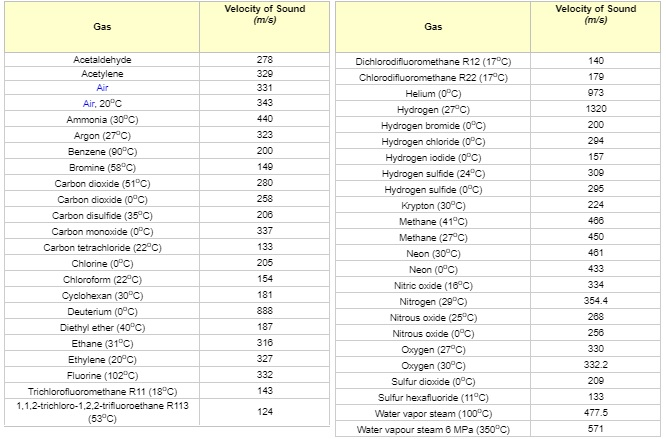
\includegraphics[scale=1.16]{images/Tabela vgas.jpg}
  \caption{Tabela de velocidades do som em diferentes gases a diferentes temperaturas}
\end{figure}


\begin{figure}[H]
  \centering
  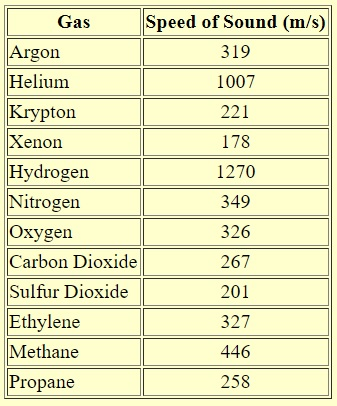
\includegraphics[scale=1.25]{images/Tabela vgas2.jpg}
  \caption{Tabela de velocidades do som em diferentes gases a 20°C e 1 atm}
\end{figure}

Baseando-nos nas tabelas encontradas, pudemos supor que o gás que foi utilizado no experimento foi o gás \textbf{Hélio}.\\

Pudemos pressupor isso, comparando a velocidade do som obtida por nós experimentalmente $v_{exp}$ com a velocidade tabelada do som nos diferentes gases nobres.

\[v_{exp} = 920 \pm 4 m/s\]
\[v_{helio} = 1007 m/s \  a \ 20^\circ C \  e  \  v_{helio} = 973 m/s\ a \ 0^\circ C\]

Dessa forma, como o ambiente do teste estava a uma temperatura maior que 0°C, assumiremos o valor da velocidade do som no hélio a 20°C, em nossas análises.

\[ \frac{v_{exp}}{v_{helio}}=\frac{920}{1007} \ \approx \ 0,9136 \ \approx \ 91,36\%  \]

Comparando os valores, temos que nossa velocidade experimental é aproximadamente 91,36 \% do valor da velocidade do som no hélio, o que representa um resultado consideravelmente bom, em se tratando de um experimento no qual nem tudo é perfeitamente "ideal".\\ 

Além disso, algumas análises, como por exemplo, o fato de o gás Hélio ser o gás nobre de mais fácil obtenção, não sendo algo muito difícil adquiri-lo. \\

Desse modo, concluímos que o gás nobre \textbf{Hélio} era o gás presente no tubo do experimento.  
